\documentclass[conference]{IEEEtran}
\usepackage{graphicx} % Required for inserting images
\usepackage{epstopdf}
\usepackage{float}
\usepackage{verbatim}
\usepackage{array}
\usepackage{authblk}
% \usepackage{IEEEtrantools}
\usepackage[
    backend=biber,
    style=ieee,
  ]{biblatex}
\addbibresource{additional.bib}  % Additional papers (those not found in SLR)
\usepackage{svg}

\usepackage{xcolor}
\usepackage{longtable}

\begin{document}

\title{Performance Analysis of Cache Size and Set-Associativity Using gem5}

\author[1]{Clayton Asada}
\author[2]{Joseph Chorbajian}
\author[3]{Ilmaan Zia}

\affil[1,2,3]{Computer Engineering and Computer Science, California State University Long Beach}

\date{February 2023}



\maketitle



\begin{abstract}
% TODO: Maybe include most prominent results/analyses in abstract?

\emph{Keywords - } Cache, Size, Associativity, Replacement Policy, gem5, Simulation, Configuration, Miss rate
\end{abstract}

% THIS IS LEFT HERE AS AN EXAMPLE/TEMPLATE FOR INCLUDING PICTURES
% \begin{figure}[H]
%     \centering
%     \includegraphics[width=0.45\textwidth]{images/EmpC1-Training}
%     \caption{Amount of training provided}
%     \label{fig:EmpC1-Training}
% \end{figure}

%\begin{table}
%    \centering
%    \begin{tabular}{| m{1.6cm} | m{.75cm} | m{.75cm} | m{.8cm} | m{2.6cm} |}
%        \hline
%        \textbf{Benchmarks} & \textbf{Cache Size} & \textbf{Block Size} & \textbf{Set Assoc.} & \textbf{Replacement Policy} \\ \hline
%        Dijkstra    &   16kB  &   32    &  1   &    Least Recently Used     \\ \hline
%        Sha         &   32kB  &   64    &  2   &    Random                  \\ \hline
%        Rijndael    &   64kB  &         &  4   &    First In First Out      \\ \hline
%                    &         &         &  8   &                            \\ \hline
%    \end{tabular}
%\end{table}

\section{Introduction}
Cache performance is a critical factor in the overall performance of modern computer systems. Cache design involves balancing the trade-offs between cache size, associativity, and replacement policies to achieve optimal performance for a given workload. Simulation tools such as gem5 and SimpleScalar provide powerful means for evaluating cache performance, allowing researchers to explore a wide range of cache configurations and workloads in a controlled environment.

In this paper, we present a study of cache performance using the gem5 simulator to model various single-core CPU cache configurations. Our aim is to compare the results of our study with the results of a previous study that used the SimpleScalar simulator. The previous study focused on the impact of cache size, block size, and associativity on miss rate performance, while our study explores the impact of replacement policies in addition to cache size, block size, and associativity.

Our research uses three benchmarks to evaluate cache performance, from SPEC95 benchmarks to stress different aspects of the memory hierarchy. We compare our results with those of the previous study, which used a total of 5 benchmarks from SPEC95 benchmarks designed to stress the instruction cache and data cache separately. The shared benchmarks were Dijkstra, Sha, and Rijndael. The additonal benchmarks from the previous study are Go and Compress.

The use of different simulators and benchmarks provides an opportunity to compare and contrast the results of our study with those of the previous study. It also allows us to evaluate the effectiveness of gem5 in modeling cache performance compared to SimpleScalar. Our study provides insights into the impact of replacement policies on cache performance, which was not explored in the previous study.

In conclusion, our research aims to contribute to the understanding of cache performance and design using simulation tools. By comparing the results of our study with those of the previous study, we hope to provide a comprehensive picture of cache performance across different simulators and benchmarks. We also hope to demonstrate the effectiveness of gem5 in modeling cache performance and guide future research in this important area.

\section{Motivation}
The design and optimization of cache performance is critical to the overall performance of modern computer systems. Cache performance can significantly impact system performance and energy efficiency, especially in memory-intensive workloads. Therefore, understanding the trade-offs between cache size, associativity, and replacement policies is crucial in designing effective caches.

Simulation tools such as gem5 and SimpleScalar provide powerful means for evaluating cache performance. However, there is a need to evaluate and compare the effectiveness of these simulators in modeling cache performance. Additionally, there is a need to explore the impact of replacement policies on cache performance, which was not studied in the previous research did not cover.

Our research aims to contribute to the understanding of cache performance and design by using the gem5 simulator to model various single-core CPU cache configurations. We aim to evaluate the effectiveness of gem5 in modeling cache performance compared to SimpleScalar, which was used in a previous study. We also aim to explore the impact of replacement policies on cache performance in addition to cache size and associativity. By comparing the results of our study with those of the previous study, we hope to provide a comprehensive picture of cache performance across different simulators and identify any differences in their respective results.

Our research has the potential to inform cache design and optimization, as well as guide future research in this area. By understanding the impact of cache size, associativity, and replacement policies on performance, we can design more effective caches that improve system performance and energy efficiency. Furthermore, by evaluating the effectiveness of simulation tools such as gem5 and SimpleScalar, we can improve the accuracy and efficiency of cache performance modeling.

\section{Related Work}

The importance of cache performance in modern computer systems has been widely recognized in the computer architecture research community. As a result, cache design has been extensively studied and optimized to improve system performance. Research studies have explored configurations of cache designs through simulation for decades.

For example, many researchers explored the trade-offs between cache replacement policies. Al-Zoubi et. al.\cite{10.1145/986537.986601} explored cache replacement policies on the CPU2000 benchmark suite using SimpleScalar in 2004. They found that LRU and LRU-based specifically, pseudo-LRU replacement policies performed best. Panda et. al.\cite{7806218} shows modern LRU-based replacement policies outperforming pseudo-LRU using SimpleScalar, this time using the CPU2006 benchmarks.

The capacity of the cache has been explored in Ma et. al.\cite{5260945}. Like other researchers, they use SimpleScalar to determine miss rates across multiple benchmarks in SPEC2000. They noticed that a larger L1 cache size improves significantly when the cache size is small, but gradually decreases as the cache gets bigger. Ullah et. al.\cite{8975563} expands on this by creating a 2:1 cache rule of thumb, where they claim that the miss rates of $n$ cache size and $x$ associativity is equivalent to the miss rates on a configuration with $n/2$ cache size and $2x$ associativity.

% TODO: Determine whether the below is best fit in Related Work or in some other section

Many simulations of miss rates for various processor configurations use SimpleScalar\cite{10.1145/268806.268810} as their simulator of choice. Original versions of SimpleScalar used its own instruction set architecture derived from MIPS-IV ISA\cite{10.1145/268806.268810} and may not necessarily model real-world processors accurately. While there has been significant research on porting SimpleScalar to different architectures, such as PowerPC, x86, and ARM\cite{10.1145/986537.986601} (with ARM being verified as cycle-accurate\cite{CHUNG2006137}), most research papers on simulating miss rates do not specify the environment or instruction set architecture it was ran on.

\section{Research methodology}
In this research, we use the gem5 simulator to model various single-core CPU cache configurations and evaluate their performance under different workloads. We describe the experimental methodology below.

Hardware and Software Configuration:
We use a Linux-based system for our experiments as that is a base requirement for the gem5 simulator. Additionally the research team purposefully used different types of hardware and operating systems to run the simulations to determine if there were any inconsistencies in the gem5 simulator. Two desktop computers, one operating on Ubuntu 22.04 and the other Debian distro, and a third laptop using WSL were used to run the gem5 simulations. We use gem5 version 20.0.0 for our simulations.

Workloads:
We use a variety of benchmark workloads to evaluate the performance of different cache configurations. The specific benchmarks used in this research are Dijkstra, Sha, and Rijndael from the SPEC95 benchmark quite. The previous paper used two additional workloads, Go and Compress.

Cache Configurations:
We evaluate several cache configurations with different sizes, different block sized, associativity, and replacement policies. As seen in the cache sizes configurations used were 16kB, 32kB, and 64kB. Cache block sizes were configuratble to 32 bytes and 64 bytes. The final configurations that were used for the original research was set associativities of 1, 2, 4, and 8. The additional configuration used in this study beyond what the original tested are following replacement policies, least recently used, random replacement, and first in first out replacement policy.

We use the findings of the previous research paper as a baseline for comparison of each unique combination of configurations.

Simulation Setup:
We use gem5's full-system mode to simulate our experiments. In this mode, the entire system, including the CPU, cache, and memory hierarchy, is simulated. We run each workload multiple times to ensure the stability of the results and use a warm-up period to ensure that the cache is populated before we start collecting performance data.

Performance Metrics:
We collect several performance metrics, including execution time, instruction throughput, and cache hit rate. We also collect cache miss rate, cache eviction rate, and average memory access latency to provide a more detailed analysis of cache behavior.

Statistical Analysis:
We use statistical analysis to compare the performance of different cache configurations. We use the t-test to determine if there are statistically significant differences between the performance of different configurations. We also use analysis of variance (ANOVA) to determine the impact of different cache parameters on performance.

In summary, our experimental methodology involves using the gem5 simulator to evaluate various single-core CPU cache configurations under different workloads. We use a range of performance metrics to compare the performance of different configurations and use statistical analysis to determine the significance of our results.

\section{Results}
In this section the results of each simulation, by benchmark, will be review and thoroughly discussed and analyzed. The target benchmarks are Sha, Dijkstra, and Rijndael.

\subsection{Sha Benchmark}



\subsection{Dijkstra Benchmark}

In the following section contains the results of simulations using various caceh configurations and the Dijkstra benchmark. Each figure show a different aspect of the cache configurations.

\begin{figure}[H]
  \centering
  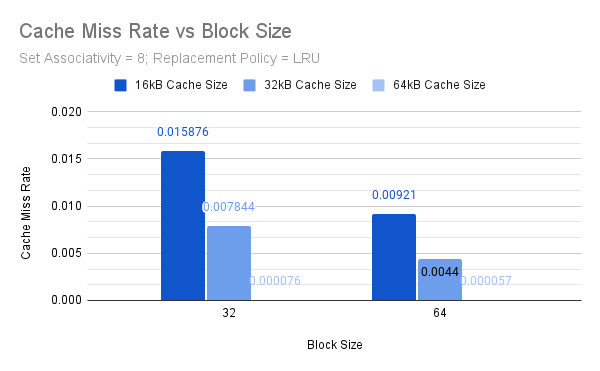
\includegraphics[width=0.45\textwidth]{dijkstraFigures/CacheMissRatevsBlockSize.png}
  \caption{Miss Rate Comparison of Block Size for Dijkstra Benchmark}
  \label{fig:EmpC1-Training}
\end{figure}

The above figure depicts the D-cache miss rate with respect to different overall cache sizes and block size. In addition the set associativity is fixed at 8-way and and the replacement policy is set to Least Recently Used (LRU). These values have been fixed to show only the effects of cache size and block size on D-cache miss rate. 

Significant difference are seen in performance from both cache size changes and block size. For a 16kB cache, changing the block size from 32 bytes to 64 bytes, is nearly as effective at reducing miss rate as doubling the cache size and maintaining the same block size. This finding did not true from 32kB cache to 64kB cache, but across each configuration, doubling the block size resulted in nearly a 50\% reduction in D-cache miss rate.

While Dijkstra benchmark can be very compute heavy, having to calculate distances for many pairs of nodes, it appears that the 100x100 adjacency matrix was still too small test the effectiveness of cache configurations on a 64kB cache. The minute miss rate shown ing the above figure indicates that a significant majority of the D-cache misses consist of conpulsory cache misses, and once the data is loaded the cache can hold all of the data throughout execution.

\begin{figure}[H]
  \centering
  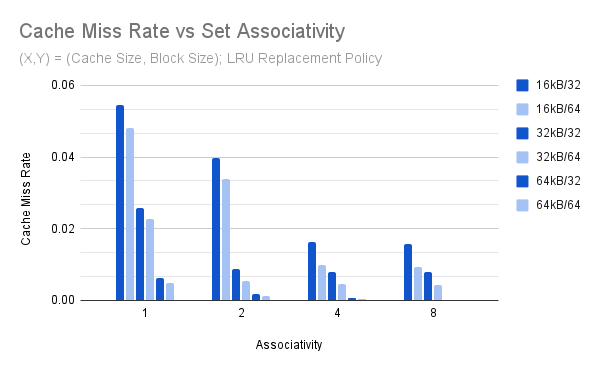
\includegraphics[width=0.45\textwidth]{dijkstraFigures/CacheMissRatevsSetAssociativity.png}
  \caption{Miss Rate Comparison of Set Associativity for Dijkstra Benchmark}
  \label{fig:EmpC1-Training}
\end{figure}

Here we allow ourselves to vary more parts of the configuration. Having only cache replacement policy as a fixed value set to LRU. By comparing neighboring dark(left) and light(right) columns we can compare the effects of cache block size changes for a given set associativity. Looking at the first two columns on the left, we can see that doubling block size does not have nearly the same effect at low associativity, miss reduction of 16\%, as it does with high associativity, reduction of 42\%.

Additionally with this graph we can compare miss rates for the 2:1 rule of thumb in cache configurations. This rule states that doubling associativity and halving the cache size should result in equivalent D-cache miss rates. By inspecting column 3 of set associativity 2 groups, we find the following cache configuartion, Cache Size: 32kB, Block Size: 32 bytes and Replacement Policy: LRU. Next observe column 1 of group 4-way set associativy, the cache configuration is as follows, Cache Size: 16kB, Block Size: 32 bytes and Replacement Policy: LRU. By the rule of thumb we should see that these two columns and configurations resulting in equivalent cache miss rate. This is not what is obversed though. In our simulations using the gem5 simulator and Dijkstra benchmark, here specifically, there is no 2:1 rule of thumb present in any pair of applicable configurations.

\begin{figure}[H]
  \centering
  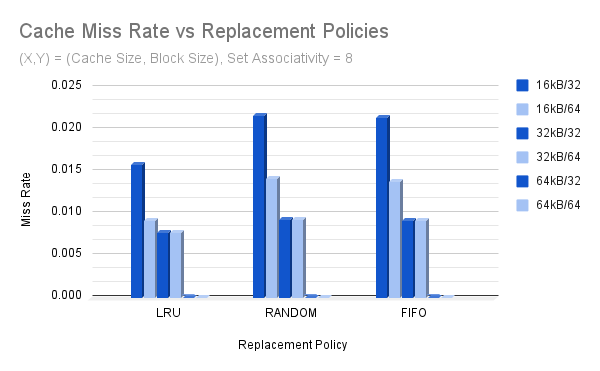
\includegraphics[width=0.45\textwidth]{dijkstraFigures/CacheMissRatevsReplacementPolicies.png}
  \caption{Miss Rate Comparison of Replacement Policies for Dijkstra Benchmark}
  \label{fig:EmpC1-Training}
\end{figure}

Finally we example replacement policy's effects on cache miss rate. In the figure we have fixed set associativity at 8-way, specifically for the replacement policy to have as many options as possible for choosing a victim block. Here we observe significantly reduced returns as compared to other cache configuration changes. LRU does perform best in almost every case, there were two outlier scenarios of 16kB cache size, block size 32 bytes with 2-way and 4-way associativity having greater performance with Random replacement policy. Overall, First In First Out and Random replacement policies appear equivalent in efficacy. 

While LRU policy does perform best in general across the board implementation of a more complex replacement policy, LRU vs FIFO or Random, may not be worth the effort for hardware architects. Particularly in embedded systems where size, power, and cost are off the utmost importance, these findings indicate that replacement policy would be a good starting point for savings across these three metrics.

\begin{figure}[H]
  \centering
  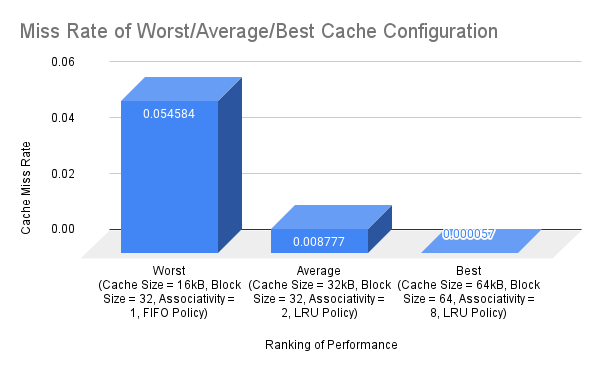
\includegraphics[width=0.45\textwidth]{dijkstraFigures/MissRateofWorstAverageBestCacheConfiguration.png}
  \caption{Miss Rate of Worst, Average, and Best Performing Cache Configurations for Dijkstra Benchmark}
  \label{fig:EmpC1-Training}
\end{figure}

In conclusion of Dijkstra benchmark analysis, the above chart plots the miss rate of the worst, average, and best performing cache configurations. For the Dijkstra benchmark, bigger meant better. Bigger Cache, bigger block size and higher associativity were all guarantees of increased performance and significant reductions in miss rate. Many of the previous charts were unable to effectively depict the miss rate of 64kB cache because its miss rates were so minute.

\subsection{Rijndael Benchmark}



\section{Discussion}


\section{Future Work}
The use of gem5 to model various single-core CPU cache configurations provides a powerful tool for evaluating cache performance. Our research has shown that different cache configurations can have a significant impact on performance, and that using simulation tools such as gem5 can provide detailed insights into cache behavior.

There are several directions for future research in this area:

Multi-core CPU Cache Configurations: In this study, we focus on single-core CPU cache configurations. However, multi-core CPUs are becoming increasingly common, and cache design for multi-core CPUs is a complex and challenging area of research. Future studies could use gem5 to model various multi-core CPU cache configurations and evaluate their performance under different workloads.

Machine Learning Techniques: Recent research has explored the use of machine learning techniques to optimize cache performance. These techniques involve using machine learning algorithms to predict cache behavior and optimize cache configurations. Using gem5 to evaluate these techniques can help identify their strengths and weaknesses and guide future research in this area.

Emerging Memory Technologies: Emerging memory technologies, such as phase-change memory (PCM) and resistive random-access memory (RRAM), have the potential to revolutionize cache design. These technologies have different performance characteristics than traditional memory technologies, and designing caches that can take advantage of their unique properties is an area of active research. Future studies could use gem5 to evaluate cache designs that incorporate emerging memory technologies.

Energy-Efficient Caches: Energy efficiency is becoming an increasingly important consideration in cache design. Caches are power-hungry components of the memory hierarchy, and designing energy-efficient caches is essential to reduce power consumption and improve battery life. Future studies could use gem5 to evaluate energy-efficient cache designs, such as cache compression and cache bypassing techniques.

In conclusion, the use of gem5 to model various single-core CPU cache configurations provides a powerful tool for evaluating cache performance. Future research in this area could explore multi-core CPU cache configurations, machine learning techniques, emerging memory technologies, and energy-efficient caches. These studies could provide valuable insights into cache design and help improve the performance and energy efficiency of modern computer systems.

\section{Conclusion}
In this research, we have used the gem5 simulator to model various single-core CPU cache configurations and evaluated their performance using several benchmarks. We compared our results with those of a previous study that used the SimpleScalar simulator to evaluate cache performance. Our research aimed to contribute to the understanding of cache performance and design, as well as evaluate the effectiveness of different simulators in modeling cache behavior.

Our study found that the performance of different cache configurations varied significantly depending on the workload characteristics. We observed that the impact of replacement policies on cache performance was insignificant, with the LRU policy outperforming the FIFO and Random policies in most cases.

Our results differed significantly from those of the previous study, which focused on the impact of cache size and associativity on performance using the SimpleScalar simulator. We found that the performance of cache configurations varied depending on the simulator. Our findings suggest that the gem5 simulator may be more effective in modeling cache behavior of modern CPU's compared to SimpleScalar.

Our research has several implications for cache design and optimization. By understanding the impact of different cache configurations on performance, designers can improve system performance and energy efficiency. Our findings also have implications for the use of simulation tools in cache performance modeling, highlighting the need for careful selection of simulator and benchmark suite.

In conclusion, our research has contributed to the understanding of cache performance and design using the gem5 simulator. Our results highlight the significant differences in cache performance between different simulators and benchmark suites. We hope that our findings will guide future research in cache design and optimization and improve the accuracy and efficiency of cache performance modeling.

\printbibliography
\end{document}
